\documentclass[12pt]{article}
\usepackage[margin=1in]{geometry}
\usepackage{setspace}
\doublespacing
\usepackage{float}
\usepackage{graphicx}
\graphicspath{{./images/}}
\usepackage{subcaption}
\PassOptionsToPackage{hyphens}{url}\usepackage{hyperref}
\hypersetup{
    colorlinks,
    citecolor=black,
    filecolor=black,
    linkcolor=black,
    urlcolor=black
}

\usepackage{xcolor}
\usepackage{listings}
% horizon bright from <https://gogh-co.github.io/Gogh>
\definecolor{codegreen}{HTML}{1D8991}
\definecolor{codelightgreen}{HTML}{1EB980}
\definecolor{codegrey}{HTML}{1A1C23}
\definecolor{codelightgrey}{HTML}{5D5E63}
\definecolor{codemagenta}{HTML}{DA103F}
\definecolor{codebackground}{HTML}{FDF0ED}
\lstdefinestyle{mystyle}{
  backgroundcolor=\color{codebackground},
  commentstyle=\color{codelightgrey},
  keywordstyle=\color{codemagenta},
  numberstyle=\ttfamily\tiny\color{codegrey},
  stringstyle=\color{codegreen},
  basicstyle=\ttfamily\footnotesize,
  breakatwhitespace=false,
  breaklines=true,
  captionpos=b,
  keepspaces=true,
  numbers=left,
  numbersep=5pt,
  showspaces=false,
  showstringspaces=false,
  showtabs=false,
  tabsize=2
}

\lstset{style=mystyle}

\title{An Analysis of Year 2 Siege: Velvet Shell}
\author{Andy Ha}
\date{}

\renewcommand*\contentsname{Table of Contents}

\begin{document}
%%%%%%%%%%%%%%%%%%%%%%%%%%%%%%%%%%%%%%%%%%%%%%%%%%%%%%%%%%%%%%%%%%%%%%%%%%%%%%%%%%%%%%%%%%%%%%%%%%%%
%%%%%%%%%%%%%%%%%%%%%%%%%%%%%%%%%%%%%%%%%%%%%%%%%%%%%%%%%%%%%%%%%%%%%%%%%%%%%%%%%%%%%%%%%%%%%%%%%%%%
% TITLE
%%%%%%%%%%%%%%%%%%%%%%%%%%%%%%%%%%%%%%%%%%%%%%%%%%%%%%%%%%%%%%%%%%%%%%%%%%%%%%%%%%%%%%%%%%%%%%%%%%%%
%%%%%%%%%%%%%%%%%%%%%%%%%%%%%%%%%%%%%%%%%%%%%%%%%%%%%%%%%%%%%%%%%%%%%%%%%%%%%%%%%%%%%%%%%%%%%%%%%%%%
\maketitle


%%%%%%%%%%%%%%%%%%%%%%%%%%%%%%%%%%%%%%%%%%%%%%%%%%%%%%%%%%%%%%%%%%%%%%%%%%%%%%%%%%%%%%%%%%%%%%%%%%%%
%%%%%%%%%%%%%%%%%%%%%%%%%%%%%%%%%%%%%%%%%%%%%%%%%%%%%%%%%%%%%%%%%%%%%%%%%%%%%%%%%%%%%%%%%%%%%%%%%%%%
% TABLE OF CONTENTS
%%%%%%%%%%%%%%%%%%%%%%%%%%%%%%%%%%%%%%%%%%%%%%%%%%%%%%%%%%%%%%%%%%%%%%%%%%%%%%%%%%%%%%%%%%%%%%%%%%%%
%%%%%%%%%%%%%%%%%%%%%%%%%%%%%%%%%%%%%%%%%%%%%%%%%%%%%%%%%%%%%%%%%%%%%%%%%%%%%%%%%%%%%%%%%%%%%%%%%%%%
\tableofcontents
\newpage


%%%%%%%%%%%%%%%%%%%%%%%%%%%%%%%%%%%%%%%%%%%%%%%%%%%%%%%%%%%%%%%%%%%%%%%%%%%%%%%%%%%%%%%%%%%%%%%%%%%%
%%%%%%%%%%%%%%%%%%%%%%%%%%%%%%%%%%%%%%%%%%%%%%%%%%%%%%%%%%%%%%%%%%%%%%%%%%%%%%%%%%%%%%%%%%%%%%%%%%%%
% INTRODUCTION
%%%%%%%%%%%%%%%%%%%%%%%%%%%%%%%%%%%%%%%%%%%%%%%%%%%%%%%%%%%%%%%%%%%%%%%%%%%%%%%%%%%%%%%%%%%%%%%%%%%%
%%%%%%%%%%%%%%%%%%%%%%%%%%%%%%%%%%%%%%%%%%%%%%%%%%%%%%%%%%%%%%%%%%%%%%%%%%%%%%%%%%%%%%%%%%%%%%%%%%%%
\section{Introduction}
Tom Clancy's Rainbow Six Siege is an online multiplayer, 5v5 videogame developed and published by Ubisoft.
The game has seen years of support having been published in December 2015 and still receiving updates, with the most recent major update being released this month, December 2024.
Over its nine years, the community has enjoyed many content releases and data analyses.
In the game's second year, during the season titled ``Operation: Velvet Shell'', Ubisoft released some of its more in-depth player-collected data for community consumption, giving a previously unknown glimpse into how players played in the Ranked playlist.
While there hasn't been a second such release of data in the seven years since, it is still an interesting source to view how play was like.

The objective of this project is to simply learn from the dataset, to experiment with models using player data.
This comes from the researcher's simple interest and love of the game, having been playing since not long after the dataset was released.
The aim is to approach the dataset as a regular player would, asking questions an average person would ask.
The end result should be not too dissimilar to what a person would think about and conclude when asking about specific things about the game's player base.

The project source code can be found in this GitHub repository:
\url{https://github.com/Magnetize8953/ml-analysis-of-siege}

\newpage

\subsection{Data}
The datasets that were released by Ubisoft in this season consisted of player loadout selections, player objective and operator selections, and round-by-round performance records.
The files ranged from 40 megabytes to nearly 20 gigabytes.
Due to size and computational limits, the medium-sized dataset was chosen, the player objective and operator selections.
This dataset came in at 804 megabytes and over 8,700,000 data samples and 12 features.

For some additional background, Rainbow Six Siege, or just Siege, has its gameplay split between gamemodes, maps, and operators, each offering a different experience.
The gamemodes available in the Ranked playlist back in Velvet Shell were bomb, secure area, and hostage.
The possible maps in play numbered in at 16.
Together, each map in each gamemode featured a number of objectives that could be selected by one team to defend and have the other attack.
These two sides, Defenders and Attackers, have their own distinctive operators, in-game characters with unique special abilities.
All together, these allow players to synthesise strategies to get kills and achieve round and match wins.
Given enough wins and losses, players are given, as of Velvet Shell, one of seven ranks.

The dataset includes all the information explained in the game background for a given day over the course of about a week.
What is important to note is that a sample is equivalent to one day of a given combination.
For example, one sample could be of Bronze PC players playing the Fuze attacking operator on Chalet on the hostage gamemode's library objective.
For the sake of brevity, the word ``player'' will be used in reference to a data sample, but know that the sample includes more than just the player.

\newpage

\subsection{Data Analysis}
An initial visual analysis of the numerical data finds a positive correlation between each point with one another.
It is also clear that there is a clustering of samples regardless of player rank in the bottom left corner.
This would make sense, especially given the scales, that most players and combinations perform in the lower tier.
An interesting observation is that the outstanding players, those reaching the upper right of the graphs, are all of the Gold rank.
This rank is the typical, middle-of-the-pack player, the players who are capable, but not exceptional.
The likely reason for this seemingly average player reaching these peaks is because the number of people at this rank.
It isn't that the players here are exceptional; it's that there is an exceptional number of players here.
\begin{figure}[H]
	\centering
	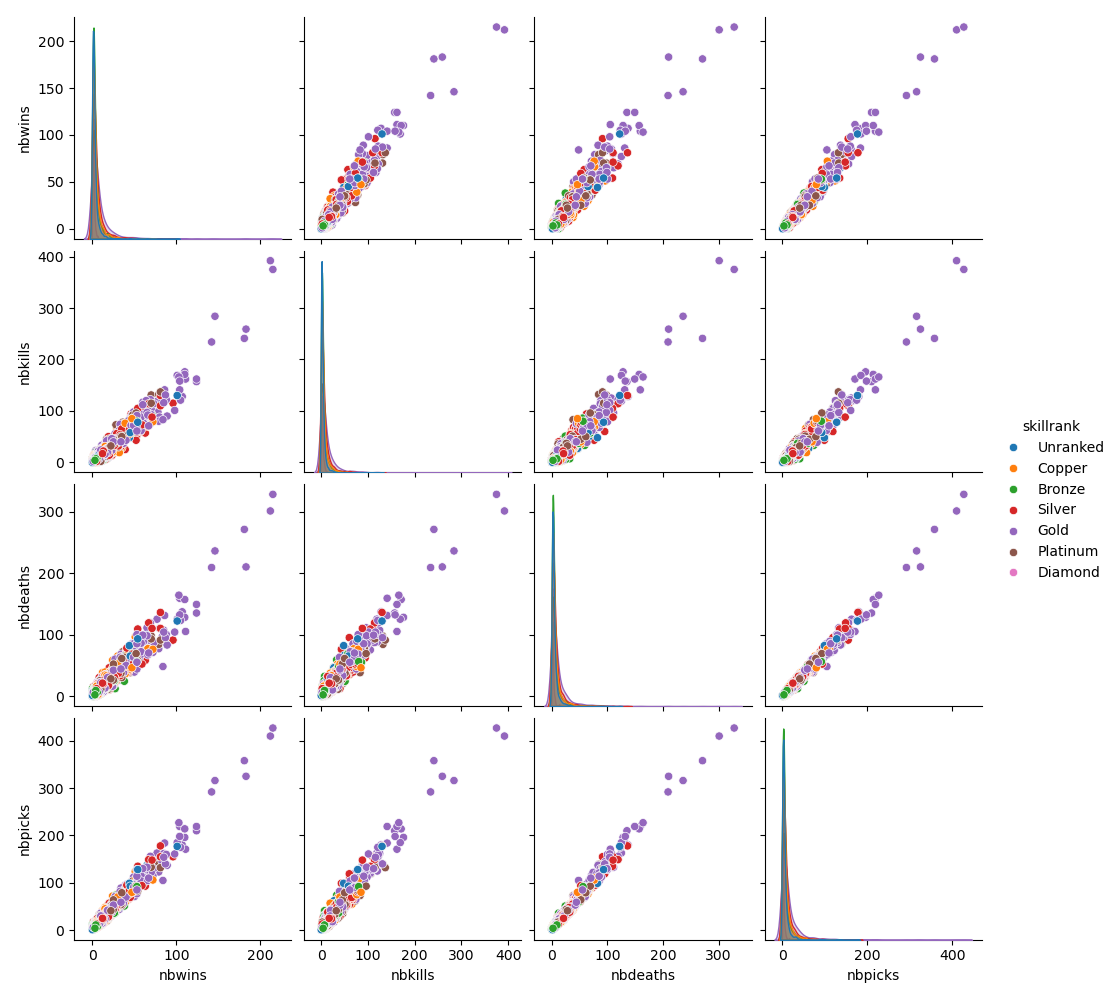
\includegraphics[width=0.85\textwidth]{wins-kills-deaths-picks-pairplot}
	\caption{Seaborn-generated PairPlot of wins, kills, deaths, and operater picks with colours corresponding to ranks}
	\label{fig:pairplot}
\end{figure}

Additional analyses were performed on player wins and kills at different ranks, in different gamemodes, and on different platforms.
This was done to get a sense of what players were included in the dataset.
From the graphs, it would appear, expectedly, that the largest group of players were ranked in Gold and those playing on PlayStation 4, though not necessarily that most players were Golds on PS4.
Additionally, the most common gamemode seemed to have been secure area.
This is an interesting observation as the second-place gamemode, bomb, is usually seen as the most competitive mode, with professional play having always been in that gamemode and a change from a few years back setting it as the only gamemode available in the Ranked playlist.
\begin{figure}[H]
	\begin{subfigure}[h]{0.49\linewidth}
		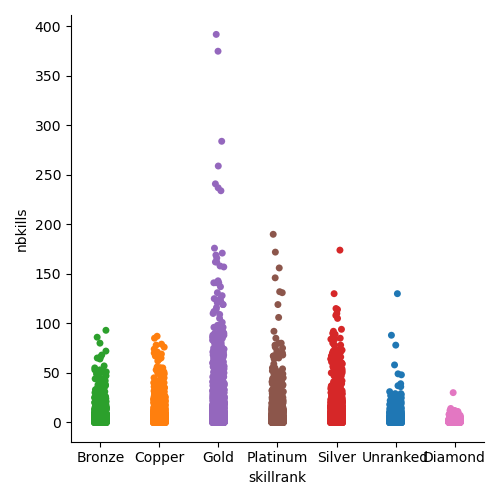
\includegraphics[width=\textwidth]{kills-rank}
		\caption{Number of kills per player rank}
	\end{subfigure}
	\hfill
	\begin{subfigure}[h]{0.49\linewidth}
		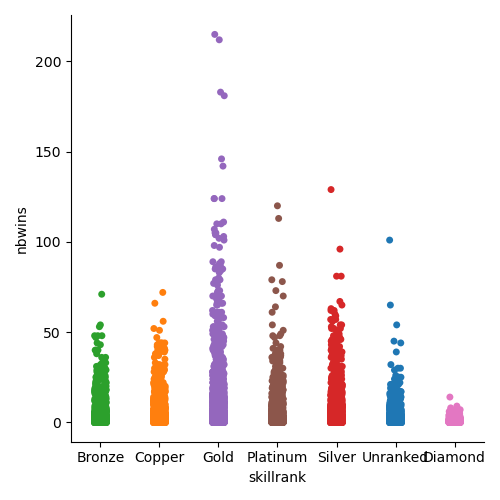
\includegraphics[width=\textwidth]{wins-rank}
		\caption{Number of round wins per player rank}
	\end{subfigure}
	\caption{Charts of player kills and round wins divided by rank}
	\label{fig:wins-kills-rank}
\end{figure}
\begin{figure}[H]
	\begin{subfigure}[h]{0.49\linewidth}
		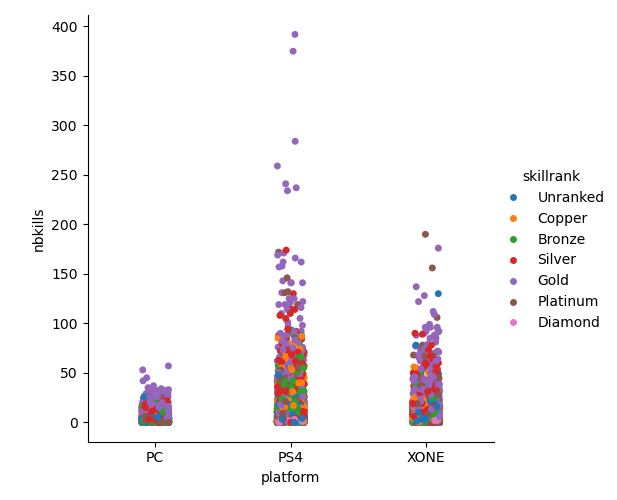
\includegraphics[width=\textwidth]{kills-platform}
		\caption{Number of kills per platform}
	\end{subfigure}
	\hfill
	\begin{subfigure}[h]{0.49\linewidth}
		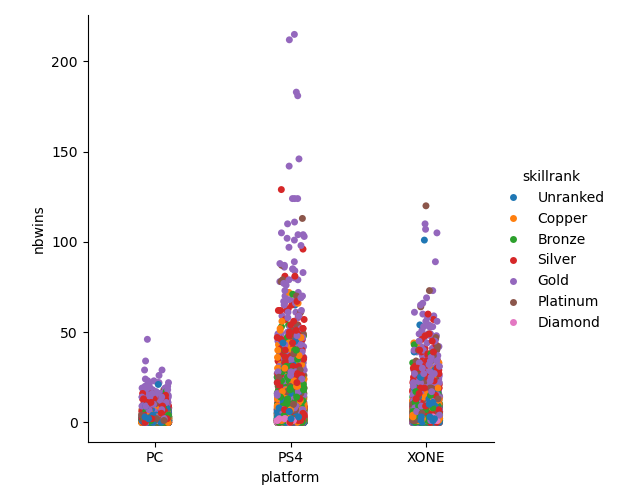
\includegraphics[width=\textwidth]{wins-platform}
		\caption{Number of round wins per platform}
	\end{subfigure}
	\caption{Charts of player kills and round wins divided by platform}
	\label{fig:wins-kills-platform}
\end{figure}
\begin{figure}[H]
	\begin{subfigure}[h]{0.49\linewidth}
		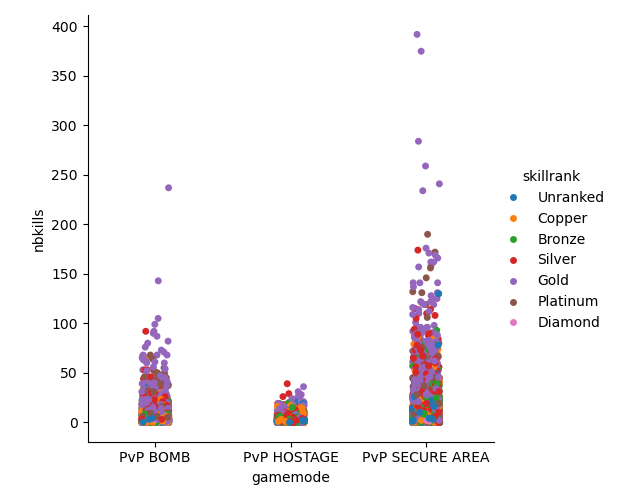
\includegraphics[width=\textwidth]{kills-gamemode}
		\caption{Number of kills per gamemode}
	\end{subfigure}
	\hfill
	\begin{subfigure}[h]{0.49\linewidth}
		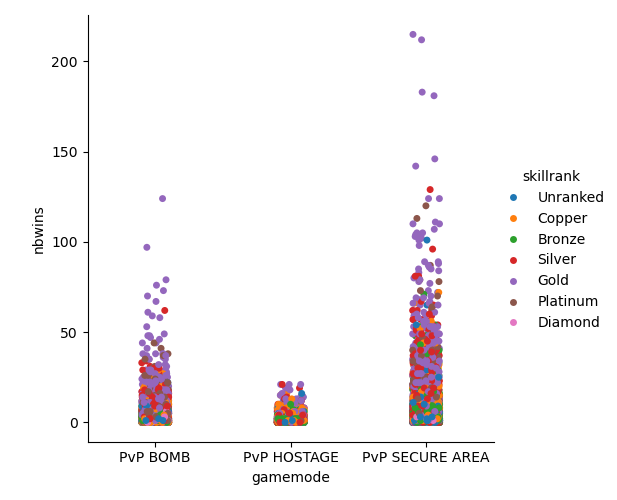
\includegraphics[width=\textwidth]{wins-gamemode}
		\caption{Number of round wins per gamemode}
	\end{subfigure}
	\caption{Charts of player kills and round wins divided by gamemode}
	\label{fig:wins-kills-gamemode}
\end{figure}

\newpage

\subsection{Data Preprocessing}
The data was preprocessed in two stages: prior to being added to the project and within the project.
The additional step of pre-project preprocessing was necessary to make the data compatible with the libraries used.
In its initial state, each data sample within the set included a non-standard hyphen character.
This character caused issues when being read by Pandas, and thus rendered the data unusable without modification.
The following command was run to clean up the data:
\begin{lstlisting}[language=Bash]
	cat -v datadump_S5_summary_objectives.csv \
	| sed 's/M-\^V //' \
	| sed 's/\^M//' > datadump_S5_summary_objectives-cleaned.csv
\end{lstlisting}

Once made possible to read, the data was entered into a Pandas DataFrame.
Only a small sample of 0.16\% of the dataset was actually saved, though, due to computational limits.
This turned out to be about 14,000 data samples across 12 features.
This was soon reduced and then increased.

One of those features was the date in which the data was collected.
As mentioned before, each sample corresponded to a collection of data for a given day.
This meant some collections would match exactly, except for the days.
To get around this unnecessary data, the column was dropped and then the numerical data was aggregated together based on shared features.
This reduced the number of samples by about 800 to 13,200.
This was not enough though.

As the data included categories in the form of written word, it was not immediately possible to pass through to machine learning libraries.
These strings had to be encoded.
One-hot encoding was chosen for its effectiveness, intuitiveness, and ability to prevent misinterpretations of higher numbers being more important, an issue with other encoding methods (Meriläinen).
The end result was 212 features, most of which were binary indicators of whether or not a certain category was found in the sample.

\newpage


%%%%%%%%%%%%%%%%%%%%%%%%%%%%%%%%%%%%%%%%%%%%%%%%%%%%%%%%%%%%%%%%%%%%%%%%%%%%%%%%%%%%%%%%%%%%%%%%%%%%
%%%%%%%%%%%%%%%%%%%%%%%%%%%%%%%%%%%%%%%%%%%%%%%%%%%%%%%%%%%%%%%%%%%%%%%%%%%%%%%%%%%%%%%%%%%%%%%%%%%%
% METHODS
%%%%%%%%%%%%%%%%%%%%%%%%%%%%%%%%%%%%%%%%%%%%%%%%%%%%%%%%%%%%%%%%%%%%%%%%%%%%%%%%%%%%%%%%%%%%%%%%%%%%
%%%%%%%%%%%%%%%%%%%%%%%%%%%%%%%%%%%%%%%%%%%%%%%%%%%%%%%%%%%%%%%%%%%%%%%%%%%%%%%%%%%%%%%%%%%%%%%%%%%%
\section{Methods and Algorithms}
Two algorithms were chosen to fit and test on this dataset: a classifier using K-Nearest Neighbour and a regression neural network.
Both were brought in from external libraries, specifically scikit-learn and TensorFlow.
While both had been previously hand-developed in coursework throughout the semester, part of the goal of this project was to learn about existing tooling and libraries and how to use them.

K-Nearest Neighbour is not really a machine learning model.
It takes in a large ``training'' dataset and then uses it to geometrically map out where a new data sample would fall.
Based on \verb`K` number of the sample's nearest neighbours would it be classified.
The reason it isn't necessarily a machine learning model is that second word, ``learning''.
The algorithm simply takes in the data, compares against a map it has made, and returns a prediction.
It doesn't learn from the initial dataset, but rather directly reads across it.
Nonetheless, this model predicts a player's platform given the rest of a data sample.
There are three possible results: PC, PlayStation 4, and Xbox One.
After testing, the model was seen performing best when comparing against 15 neighbours using a uniform weight algorithm.

The neural network, on the other hand, is a fully blown machine learning model.
It makes use of training data it is given and learns and modifies weights based on whether or not its predictions were correct.
The neural network used in this project involved four hidden layers with each layer decreasing in size by half.
It starts with the input data at 212 features and ends with seven probabilities, each corresponding to the model's confidence that the given inputs are from a certain rank.
Each of the hidden layers made use of the ReLU activation function, a common and well-performing function.
The model makes use of the Adam gradient descent optimiser and measures loss using mean square error.

\newpage


%%%%%%%%%%%%%%%%%%%%%%%%%%%%%%%%%%%%%%%%%%%%%%%%%%%%%%%%%%%%%%%%%%%%%%%%%%%%%%%%%%%%%%%%%%%%%%%%%%%%
%%%%%%%%%%%%%%%%%%%%%%%%%%%%%%%%%%%%%%%%%%%%%%%%%%%%%%%%%%%%%%%%%%%%%%%%%%%%%%%%%%%%%%%%%%%%%%%%%%%%
% RESULTS
%%%%%%%%%%%%%%%%%%%%%%%%%%%%%%%%%%%%%%%%%%%%%%%%%%%%%%%%%%%%%%%%%%%%%%%%%%%%%%%%%%%%%%%%%%%%%%%%%%%%
%%%%%%%%%%%%%%%%%%%%%%%%%%%%%%%%%%%%%%%%%%%%%%%%%%%%%%%%%%%%%%%%%%%%%%%%%%%%%%%%%%%%%%%%%%%%%%%%%%%%
\section{Results}
While it was completely possible to compare the models on the same problem, for the sake of experimentation, they were tested on different prediction problems.
As mentioned before, the KNN model predicted platform whereas the neural network predicted rank.

\subsection{K-Nearest Neighbour}
The KNN model was set up to predict a player's platform of choice.
Given all of information, the question was what platform is this player playing on?

Training was done with scikit-learn's \verb`KNeighborsClassifier` class.
It provided a pre-built solution to the KNN problem.
All that was needed was to give it data, a number of neighbours to check, and a method of weighing each neighbour.
After some simple trial and error, the best number of neighbours was determined to be 15 with a uniform weighing method.

The result of this was a 95\% accuracy rate on the testing data after training.
The following confusion matrix was produced by the testing data.
It would appear as though the model was most confused about Xbox One players, with the largest number of misclassifications coming from that platform as the true value.
It does also seem like PC-PS4 performances confused the model, with the next highest number of misclassifications being PS4 as PC.
This could indicate similar playstyles by these platforms in some cases.
The source of this is not clear by the model's results and could be a number of things, including very popular operator selections or must-have picks for a certain objective.
\begin{figure}[H]
	\centering
	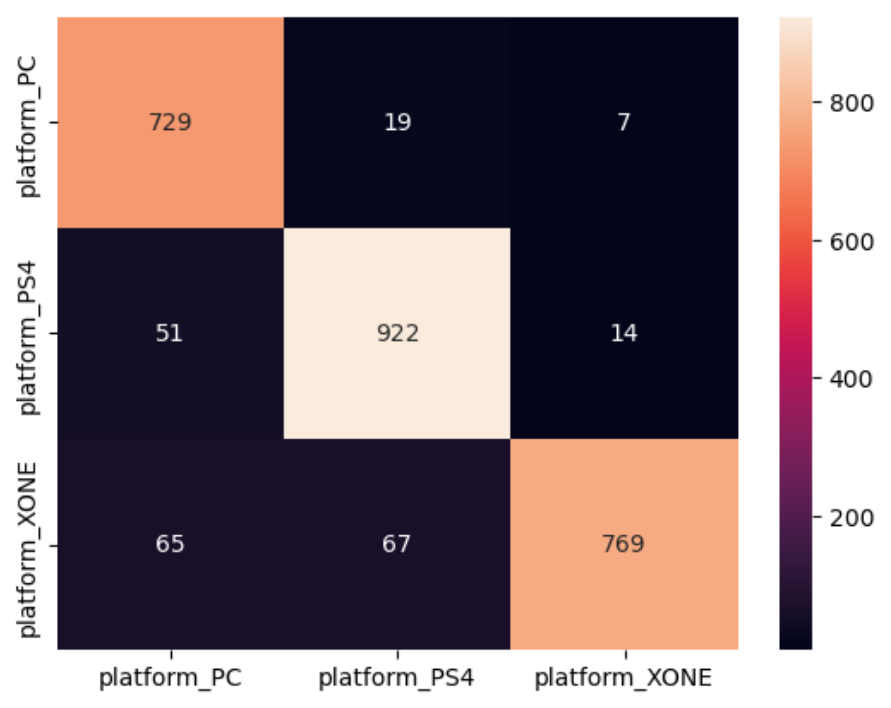
\includegraphics[width=0.7\textwidth]{knn-confusion-matrix}
	\caption{Confusion matrix of K-Nearest Neighbour model classifying platform}
	\label{fig:knn-confusion-matrix}
\end{figure}

\subsection{Neural Network}
The neural network was set up to predict something different from the KNN model.
The decision to do this was purely curiousity.
As the objective of the course project was not necessarily to compare performances of the models, this curiousity-fueled adventure was deemed acceptable by the researcher.

This model was created to predict player ranks.
The decision to go after player ranks was made due to it being a common things players wonder, often using a low rank to insult a player's performance and capabilities.
The reason it was decided to be the thing tested by the neural network was due to it being a regression model and not a simple classifier.
To mimick an average player, there can't be complete certainty, but rather a confidence level, a percentage in which the player believes this person is in a given rank.

Following common advice, the network was designed in a decrease-number-of-neurons way, with each layer cutting the number of neurons in half.
Since the input features start at 212, the first hidden layer houses 106 neurons, and this number decreases until it reaches the seven output neurons, one for each rank.
Also in line with common advice, the model makes use of the ReLU activation function for each neuron.
This was simply found to be the most performant.
Also as mentioned before, the Adam gradient descent optimiser and mean squared error loss function were used.
To keep track of how the model is performing throughout its training, the root means squared error function was used as a metric.
During its training, 10 epochs were utilised, mainly due to computational time and diminishing returns.

Speaking of diminishing returns, with 10 epochs, it was found that the training data error was stabilising at around 0.0020 loss and the validation data at even less.
\begin{figure}[H]
	\centering
	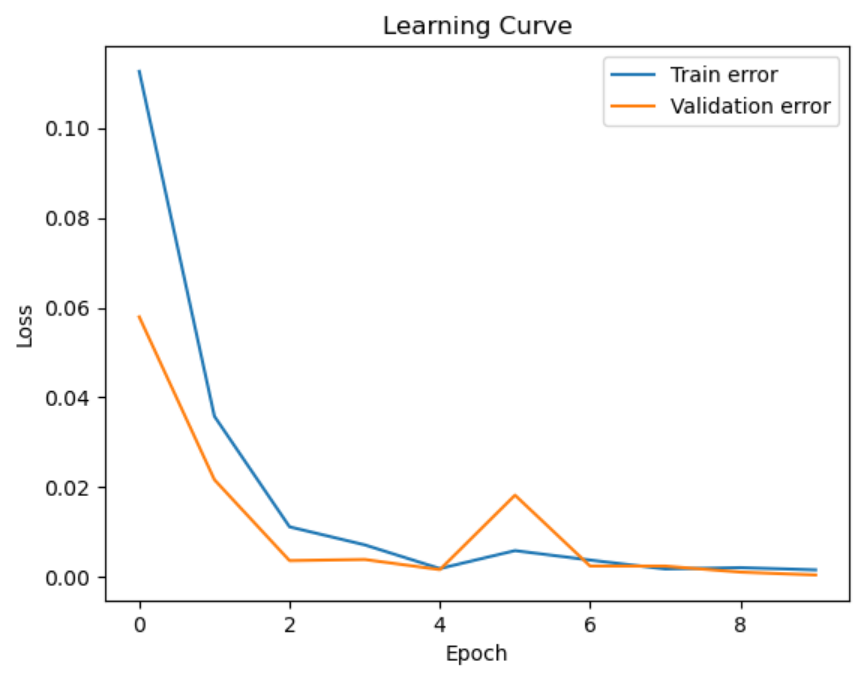
\includegraphics[width=0.7\textwidth]{nn-learning-curve}
	\caption{Learning curve of neural network training}
	\label{fig:nn-learning-curve}
\end{figure}

While accuracy was initially attempted to be calculated using the usual formula of correct over total, due to the neural network not producing binary data classifications, this was not possible.
Instead, just a confusion matrix was plotted based on the testing data.
The matrix shows 100\% accuracy by the model.
This would appear to indicate, despite the shear number of possibilities within the game, each rank is clearly separable based on selections and performance.
This is slightly surprising, once again given the shear number of possibilities within the game.
Initial expectations were for some mistakes to be made around neighbouring ranks, e.g. Golds being confused for Silvers.
This could easily be a limitation of the model and dataset; not much was actually given by the selected dataset about individual players, but rather groups of players.
\begin{figure}[H]
	\centering
	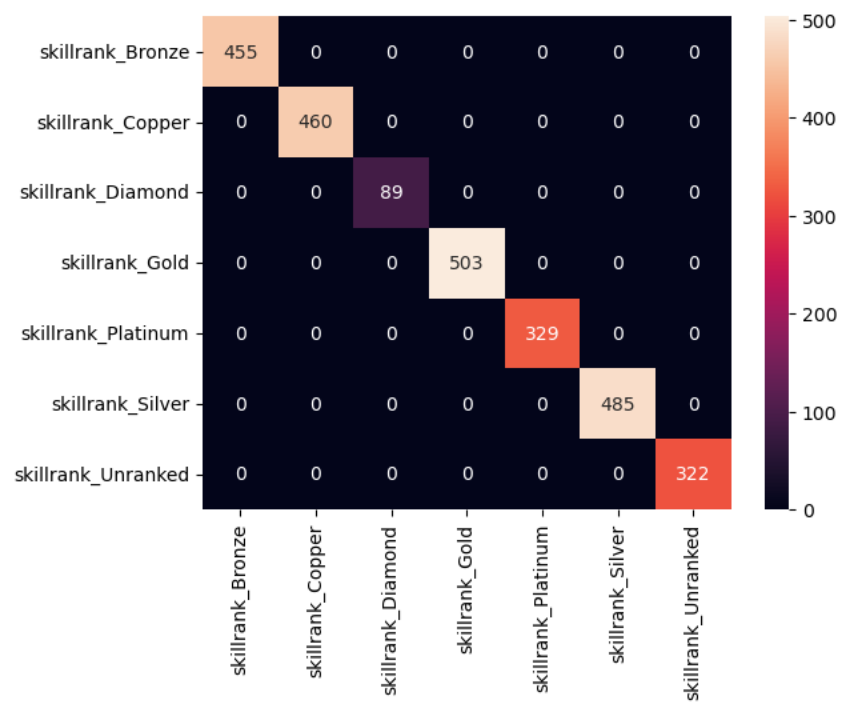
\includegraphics[width=0.7\textwidth]{nn-confusion-matrix}
	\caption{Confusion matrix of neural network regression model}
	\label{fig:nn-confusion-matrix}
\end{figure}

\newpage


%%%%%%%%%%%%%%%%%%%%%%%%%%%%%%%%%%%%%%%%%%%%%%%%%%%%%%%%%%%%%%%%%%%%%%%%%%%%%%%%%%%%%%%%%%%%%%%%%%%%
%%%%%%%%%%%%%%%%%%%%%%%%%%%%%%%%%%%%%%%%%%%%%%%%%%%%%%%%%%%%%%%%%%%%%%%%%%%%%%%%%%%%%%%%%%%%%%%%%%%%
% CONCLUSION
%%%%%%%%%%%%%%%%%%%%%%%%%%%%%%%%%%%%%%%%%%%%%%%%%%%%%%%%%%%%%%%%%%%%%%%%%%%%%%%%%%%%%%%%%%%%%%%%%%%%
%%%%%%%%%%%%%%%%%%%%%%%%%%%%%%%%%%%%%%%%%%%%%%%%%%%%%%%%%%%%%%%%%%%%%%%%%%%%%%%%%%%%%%%%%%%%%%%%%%%%
\section{Conclusion}
Overall, this was a very enjoyable project.
While there is some disappointment in the fact that this dataset is nearing its eighth anniversary, it is still great to be able to experiment on real-world data.
The dataset was a wonder to work with and provided more than enough for novice workshopping and gave insight into how players performed in years past.

Some trends discovered were of notable interest.
Xbox One players being seemingly (relatively) easily confused with PC and PlayStation 4 players was very interesting to see, especially given the inverse was not true.
Further research into this would be interesting, especially given Ubisoft's recent invention of MouseTrap, an anti-cheat system to detect console players illegally using a mouse and keyboard on their chosen platform, giving them an unfair advantage.
Additionally, the ranks being clearly distinguishable was confusing to see, though potentially understandable given the little data was given in this dataset about individual performances.
For further testing, the larger, 20 gigabyte dataset include round-by-round data would likely be a better measure.
Perhaps in that dataset it would be clearer who belongs to which rank.

\newpage


%%%%%%%%%%%%%%%%%%%%%%%%%%%%%%%%%%%%%%%%%%%%%%%%%%%%%%%%%%%%%%%%%%%%%%%%%%%%%%%%%%%%%%%%%%%%%%%%%%%%
%%%%%%%%%%%%%%%%%%%%%%%%%%%%%%%%%%%%%%%%%%%%%%%%%%%%%%%%%%%%%%%%%%%%%%%%%%%%%%%%%%%%%%%%%%%%%%%%%%%%
% REFERENCES
%%%%%%%%%%%%%%%%%%%%%%%%%%%%%%%%%%%%%%%%%%%%%%%%%%%%%%%%%%%%%%%%%%%%%%%%%%%%%%%%%%%%%%%%%%%%%%%%%%%%
%%%%%%%%%%%%%%%%%%%%%%%%%%%%%%%%%%%%%%%%%%%%%%%%%%%%%%%%%%%%%%%%%%%%%%%%%%%%%%%%%%%%%%%%%%%%%%%%%%%%
\section{References}
% manual citations because bibtex was being weird
Meriläinen, Vili. ``How to Encode Categorical Values for Multiple Columns | Scikit-Learn.'' \emph{Medium}, \url{https://medium.com/@merilainen.vili/66fd3671384b}.

\newpage


%%%%%%%%%%%%%%%%%%%%%%%%%%%%%%%%%%%%%%%%%%%%%%%%%%%%%%%%%%%%%%%%%%%%%%%%%%%%%%%%%%%%%%%%%%%%%%%%%%%%
%%%%%%%%%%%%%%%%%%%%%%%%%%%%%%%%%%%%%%%%%%%%%%%%%%%%%%%%%%%%%%%%%%%%%%%%%%%%%%%%%%%%%%%%%%%%%%%%%%%%
% ACKNOWLEDGEMENTS
%%%%%%%%%%%%%%%%%%%%%%%%%%%%%%%%%%%%%%%%%%%%%%%%%%%%%%%%%%%%%%%%%%%%%%%%%%%%%%%%%%%%%%%%%%%%%%%%%%%%
%%%%%%%%%%%%%%%%%%%%%%%%%%%%%%%%%%%%%%%%%%%%%%%%%%%%%%%%%%%%%%%%%%%%%%%%%%%%%%%%%%%%%%%%%%%%%%%%%%%%
\section{Acknowledgements}
Information and tooling used in this project were not all gathered and developed by the researcher.
The dataset comes from the Ubisoft.
Development was done in a Jupyter Notebook using the NumPy, Pandas, scikit-learn, TensorFlow, and Matplotlib libraries.
Both the libraries' classes and functions as well as their documentation were used in development.

Additionally, this project would not be possible without the teaching and assignment by Dr. Jake Lee of UNC Charlotte and my friend Devdan's support.

\newpage


\end{document}
